\documentclass[a4paper,11pt]{report}
\usepackage{chuan_math_gkt}
\usetikzlibrary{angles,quotes,intersections,patterns,decorations.pathreplacing}
\chuanexamsetup

\begin{document}
\examfontsize

\examsecret{绝密$\bigstar$启用前}

\examtitle{2020年普通高等学校招生全国统一考试（全国甲卷理科）}{数\quad 学}

\noticetitle
\begin{examnotice}
\item 答卷前，考生务必将自己的姓名、准考证号填写在答题卡上. 
\item 回答选择题时，选出每小题的答案后，用铅笔把答题卡上对应题目的答案标号涂黑. 如需改动，用橡皮擦干净后，再选涂其他答案标号. 回答非选择题时，将答案写在答题卡上. 写在本试卷上无效. 
\item 考试结束后，将本试卷和答题卡一并交回. 
\end{examnotice}

\examsection{一、选择题：本题共12小题，每小题5分，共60分. 在每小题给出的四个选项中，只有一项是符合题目要求的. }
\begin{examquestions}

\item 已知集合 $U=\{-2,-1,0,1,2,3\}$，$A=\{-1,0,1\}$，$B=\{1,2\}$，则 $\complement_U(A\cup B)=$
\fourchoices{$\{-2,3\}$}{$\{-2,2,3\}$}{$\{-2,-1,0,3\}$}{$\{-2,-1,0,2,3\}$}

\item 若 $\alpha$ 为第四象限角，则
\fourchoices{$\cos2\alpha>0$}{$\cos2\alpha<0$}{$\sin2\alpha>0$}{$\sin2\alpha<0$}

\item 在新冠肺炎疫情防控期间，某超市开通网上销售业务，每天能完成 $1200$ 份订单的配货，由于订单量大幅增加，导致订单积压. 为解决困难，许多志愿者踊跃报名参加配货工作. 已知该超市某日积压 $500$ 份订单未配货，预计第二天的新订单超过 $1600$ 份的概率为 $0.05$，志愿者每人每天能完成 $50$ 份订单的配货，为使第二天完成积压订单及当日订单的配货的概率不小于 $0.95$，则至少需要志愿者
\fourchoices{$10$名}{$18$名}{$24$名}{$32$名}

\begin{minipage}[t]{0.62\linewidth}
\item 北京天坛的圜丘坛为古代祭天的场所，分上、中、下三层，上层中心有一块圆形石板（称为天心石），环绕天心石砌 $9$ 块扇面形石板构成第一环，向外每环依次增加 $9$ 块，下一层的第一环比上一层的最后一环多 $9$ 块，向外每环依次也增加 $9$ 块，已知每层环数相同，且下层比中层多 $729$ 块，则三层共有扇面形石板（不含天心石）
\vspace{0.5em}
\end{minipage}\hfill
\begin{minipage}[t]{0.32\linewidth}
\vspace{0em}
\centering
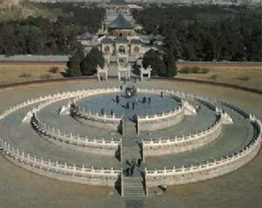
\includegraphics[width=\linewidth]{figures/2020_xkb2_li_image3.png}
\end{minipage}
\fourchoices{$3699$块}{$3474$块}{$3402$块}{$3339$块}

\newpage
\item 若过点 $(2,1)$ 的圆与两坐标轴都相切，则圆心到直线 $2x-y-3=0$ 的距离为
\fourchoices
{\tallchoice{$\dfrac{\sqrt5}{5}$}}
{\tallchoice{$\dfrac{2\sqrt5}{5}$}}
{\tallchoice{$\dfrac{3\sqrt5}{5}$}}
{\tallchoice{$\dfrac{4\sqrt5}{5}$}}

\item 数列 $\{a_n\}$ 中，$a_1=2$，$a_{m+n}=a_ma_n$，若 $a_{k+1}+a_{k+2}+\cdots+a_{k+10}=2^{15}-2^5$，则 $k=$
\fourchoices{$2$}{$3$}{$4$}{$5$}

\begin{minipage}[t]{0.62\linewidth}
\item 如图是一个多面体的三视图，这个多面体某条棱的一个端点在正视图中对应的点为 $M$，在俯视图中对应的点为 $N$，则该端点在侧视图中对应的点为
\vspace{0.5em}
\twochoices{$E$}{$F$}{$G$}{$H$}
\end{minipage}\hfill
\begin{minipage}[t]{0.28\linewidth}
\vspace{0em}
\centering
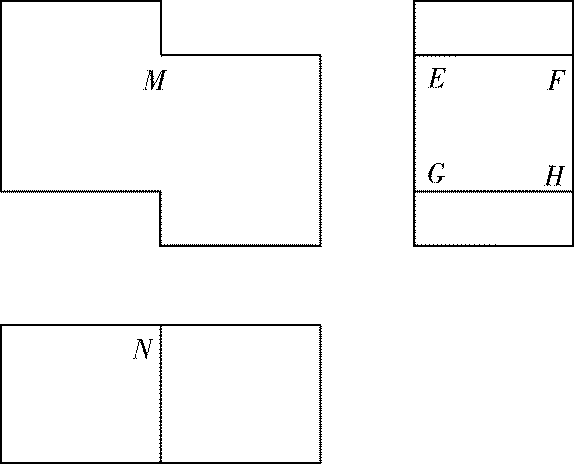
\includegraphics[width=\linewidth]{figures/2020_xkb2_li_image17.png}
\end{minipage}


\item 设 $O$ 为坐标原点，直线 $x=a$ 与双曲线 $C:\dfrac{x^2}{a^2}-\dfrac{y^2}{b^2}=1(a>0,b>0)$ 的两条渐近线分别交于 $D,E$ 两点，若 $\triangle ODE$ 的面积为 $8$，则 $C$ 的焦距的最小值为
\fourchoices{$4$}{$8$}{$16$}{$32$}

\item 设函数 $f(x)=\ln|2x+1|-\ln|2x-1|$，则 $f(x)$
\onechoices
{是偶函数，且在 $\left(\dfrac12,+\infty\right)$ 单调递增}
{是奇函数，且在 $\left(-\dfrac12,\dfrac12\right)$ 单调递减}
{是偶函数，且在 $\left(-\infty,-\dfrac12\right)$ 单调递增}
{是奇函数，且在 $\left(-\infty,-\dfrac12\right)$ 单调递减}

\item 已知 $\triangle ABC$ 是面积为 $\dfrac{9\sqrt3}{4}$ 的等边三角形，且其顶点都在球 $O$ 的球面上. 若球 $O$ 的表面积为 $16\pi$，则 $O$ 到平面 $ABC$ 的距离为
\fourchoices{$\sqrt3$}{\tallchoice{$\dfrac32$}}{$1$}{\tallchoice{$\dfrac{\sqrt3}{2}$}}

\item 若 $2^x-2^y<3^{-x}-3^{-y}$，则
\fourchoices{$\ln(y-x+1)>0$}{$\ln(y-x+1)<0$}{$\ln|x-y|>0$}{$\ln|x-y|<0$}
\item $0$--$1$ 周期序列在通信技术中有着重要应用. 若序列 $a_1a_2\cdots a_n\cdots$ 满足 $a_i\in\{0,1\}(i=1,2,\cdots)$，且存在正整数 $m$，使得 $a_{i+m}=a_i(i=1,2,\cdots)$ 成立，则称其为 $0$--$1$ 周期序列，并称满足 $a_{i+m}=a_i(i=1,2,\cdots)$ 的最小正整数 $m$ 为这个序列的周期. 对于周期为 $m$ 的 $0$--$1$ 序列 $a_1a_2\cdots a_n\cdots$，$C(k)=\dfrac1m\sum_{i=1}^m a_i a_{i+k}(k=1,2,\cdots,m-1)$ 是描述其性质的重要指标，下列周期为 $5$ 的 $0$--$1$ 序列中，满足 $C(k)\leq\dfrac15(k=1,2,3,4)$ 的序列是
\fourchoices{$11010\cdots$}{$11011\cdots$}{$10001\cdots$}{$11001\cdots$}

\end{examquestions}

\examsection{二、填空题：本题共4小题，每小题5分，共20分. }
\begin{examquestions}[start=13]

\item 已知单位向量 $\vec a,\vec b$ 的夹角为 $45^\circ$，$k\vec a-\vec b$ 与 $\vec a$ 垂直，则 $k=$ \blank.

\item $4$ 名同学到 $3$ 个小区参加垃圾分类宣传活动，每名同学只去 $1$ 个小区，每个小区至少安排 $1$ 名同学，则不同的安排方法共有 \blank 种.

\item 设复数 $z_1,z_2$ 满足 $|z_1|=|z_2|=2$，$z_1+z_2=\sqrt3+\mathrm{i}$，则 $|z_1-z_2|=$ \blank.

\item 设有下列四个命题：

$p_1$：两两相交且不过同一点的三条直线必在同一平面内. 

$p_2$：过空间中任意三点有且仅有一个平面. 

$p_3$：若空间两条直线不相交，则这两条直线平行. 

$p_4$：若直线 $l\subset$ 平面 $\alpha$，直线 $m\perp$ 平面 $\alpha$，则 $m\perp l$. 

则下述命题中所有真命题的序号是 \blank.

① $p_1\wedge p_4$；② $p_1\wedge p_2$；③ $\neg p_2\vee p_3$；④ $\neg p_3\vee\neg p_4$.
\end{examquestions}

\vspace{-0.6em}
\examsection{三、解答题：共70分. 解答应写出文字说明、证明过程或演算步骤. 第17题～第21题为必考题，每个试题考生都必须作答. 第22、23题为选考题，考生根据要求作答. }
\begin{examanswers}[start=17]

\vspace{-0.5em}
\item（12分）

$\triangle ABC$ 中，$\sin^2 A-\sin^2 B-\sin^2 C=\sin B\sin C$.

\subq{（1）}{求 $A$；}

\subq{（2）}{若 $BC=3$，求 $\triangle ABC$ 周长的最大值.}
\vspace{-1em}
\item（12分）

某沙漠地区经过治理，生态系统得到很大改善，野生动物数量有所增加. 为调查该地区某种野生动物的数量，将其分成面积相近的 $200$ 个地块，从这些地块中用简单随机抽样的方法抽取 $20$ 个作为样区，调查得到样本数据 $(x_i,y_i)(i=1,2,\ldots,20)$，其中 $x_i$ 和 $y_i$ 分别表示第 $i$ 个样区的植物覆盖面积（单位：公顷）和这种野生动物的数量，并计算得 $\sum_{i=1}^{20}x_i=60$，$\sum_{i=1}^{20}y_i=1200$，$\sum_{i=1}^{20}(x_i-\overline{x})^2=80$，$\sum_{i=1}^{20}(y_i-\overline{y})^2=9000$，$\sum_{i=1}^{20}(x_i-\overline{x})(y_i-\overline{y})=800$.

\subq{（1）}{求该地区这种野生动物数量的估计值（这种野生动物数量的估计值等于样区这种野生动物数量的平均数乘以地块数）；}

\subq{（2）}{求样本 $(x_i,y_i)(i=1,2,\ldots,20)$ 的相关系数（精确到 $0.01$）；}

\subq{（3）}{根据现有统计资料，各地块间植物覆盖面积差异很大. 为提高样本的代表性以获得该地区这种野生动物数量更准确的估计，请给出一种你认为更合理的抽样方法，并说明理由. 
附：相关系数 $r=\dfrac{\displaystyle\sum_{i=1}^{n}(x_i-\overline{x})(y_i-\overline{y})}{\sqrt{\displaystyle\sum_{i=1}^{n}(x_i-\overline{x})^2\displaystyle\sum_{i=1}^{n}(y_i-\overline{y})^2}}$，$\sqrt2\approx1.414$.}

\item（12分）

已知椭圆 $C_1:\dfrac{x^2}{a^2}+\dfrac{y^2}{b^2}=1(a>b>0)$ 的右焦点 $F$ 与抛物线 $C_2$ 的焦点重合，$C_1$ 的中心与 $C_2$ 的顶点重合. 过 $F$ 且与 $x$ 轴垂直的直线交 $C_1$ 于 $A,B$ 两点，交 $C_2$ 于 $C,D$ 两点，且 $|CD|=\dfrac43|AB|$.

\subq{（1）}{求 $C_1$ 的离心率；}

\subq{（2）}{设 $M$ 是 $C_1$ 与 $C_2$ 的公共点，若 $|MF|=5$，求 $C_1$ 与 $C_2$ 的标准方程.}

\vspace{-0.5em}
\item（12分）

如图，已知三棱柱 $ABC-A_1B_1C_1$ 的底面是正三角形，侧面 $BB_1C_1C$ 是矩形，$M,N$ 分别为 $BC,B_1C_1$ 的中点，$P$ 为 $AM$ 上一点，过 $B_1C_1$ 和 $P$ 的平面交 $AB$ 于 $E$，交 $AC$ 于 $F$.

\noindent\begin{minipage}[t]{0.69\linewidth}
\subq{（1）}{证明：$AA_1\parallel MN$，且平面 $A_1AMN\perp$ 平面 $EB_1C_1F$；}

\subq{（2）}{设 $O$ 为 $\triangle A_1B_1C_1$ 的中心，若 $AO\parallel$ 平面 $EB_1C_1F$，且 $AO=AB$，求直线 $B_1E$ 与平面 $A_1AMN$ 所成角的正弦值.}
\end{minipage}\hfill
\begin{minipage}[t]{0.25\linewidth}
\vspace{-1.2em}
\centering
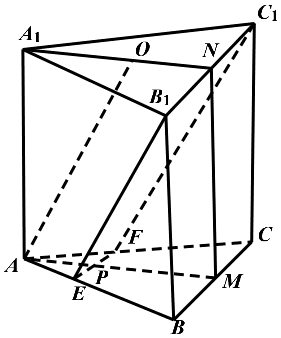
\includegraphics[width=\linewidth]{figures/2020_xkb2_li_image72.png}
\end{minipage}
\vspace{-4.9em}
\item（12分）

已知函数 $f(x)=\sin^2 x\sin2x$.

\subq{（1）}{讨论 $f(x)$ 在区间 $(0,\pi)$ 的单调性；}

\subq{（2）}{证明：$|f(x)|\leq\dfrac{3\sqrt3}{8}$；}

\subq{（3）}{设 $n\in\mathbb N^*$，证明：$\sin^2x\sin^22x\sin^24x\cdots\sin^22^nx\leq\dfrac{3^n}{4^n}$.}

\vspace{-0.5em}
\item（10分）【选修4---4：坐标系与参数方程】

已知曲线 $C_1,C_2$ 的参数方程分别为 $C_1:$\linsys{x=4\cos^2\theta\\y=4\sin^2\theta}（$\theta$ 为参数），$C_2:$\linsys{x=t+\dfrac1t\\y=t-\dfrac1t}（$t$ 为参数）. 

\subq{（1）}{将 $C_1,C_2$ 的参数方程化为普通方程；}

\subq{（2）}{以坐标原点为极点，$x$ 轴正半轴为极轴建立极坐标系. 设 $C_1,C_2$ 的交点为 $P$，求圆心在极轴上，且经过极点和 $P$ 的圆的极坐标方程.}

\vspace{-0.5em}
\item（10分）【选修4---5：不等式选讲】

已知函数 $f(x)=|x-a^2|+|x-2a+1|$.

\subq{（1）}{当 $a=2$ 时，求不等式 $f(x)\geq4$ 的解集；}

\subq{（2）}{若 $f(x)\geq4$，求 $a$ 的取值范围.}

\end{examanswers}

\end{document}